\section{Results}

\subsection{Main trajectory metrics}

\begin{table}[t]
\centering
\small
\begin{tabular}{llrrrrrr}
\toprule
Model & Condition & FTGA & Mean RTT & Tok. tax & Unres. & R@1 & R@2 \\
\midrule
GPT-4.1 nano & Baseline & 67.5 & 0.47 & 1.69 & 5.8 & 74.4 & 82.1 \\
GPT-4.1 nano & Contract & 76.7 & 0.33 & 1.34 & 4.2 & 78.6 & 82.1 \\
GPT-4.1 mini & Baseline & 75.8 & 0.28 & 1.43 & 0.8 & 89.7 & 96.6 \\
GPT-4.1 mini & Contract & 79.2 & 0.24 & 1.27 & 1.7 & 92.0 & 92.0 \\
GPT-4.1 & Baseline & 76.7 & 0.28 & 1.43 & 2.5 & 89.3 & 89.3 \\
GPT-4.1 & Contract & 93.3 & 0.15 & 1.13 & 4.2 & 37.5 & 37.5 \\
\bottomrule
\end{tabular}
\caption{Stress-pilot results. FTGA, unresolved rate, Repair@1, and Repair@2 are percentages. RTT and token tax are lower-is-better; token tax is total tokens until success or exhaustion divided by first-attempt tokens.}
\label{tab:main}
\end{table}

Table~\ref{tab:main} shows measurable baseline Re-prompt Tax for all three
models. Baseline FTGA ranges from 67.5\% for \texttt{gpt-4.1-nano} to 76.7\%
for \texttt{gpt-4.1}. The Global Interaction Contract improves FTGA for every
model, with gains of +9.2 points for nano, +3.3 points for mini, and +16.7
points for GPT-4.1. Mean RTT also falls for every model. The strongest model
reaches 93.3\% FTGA under the contract, but the unresolved rate does not vanish;
residual failures are concentrated in exact-preservation and script/register/
locale cases.

\begin{figure}[t]
\centering
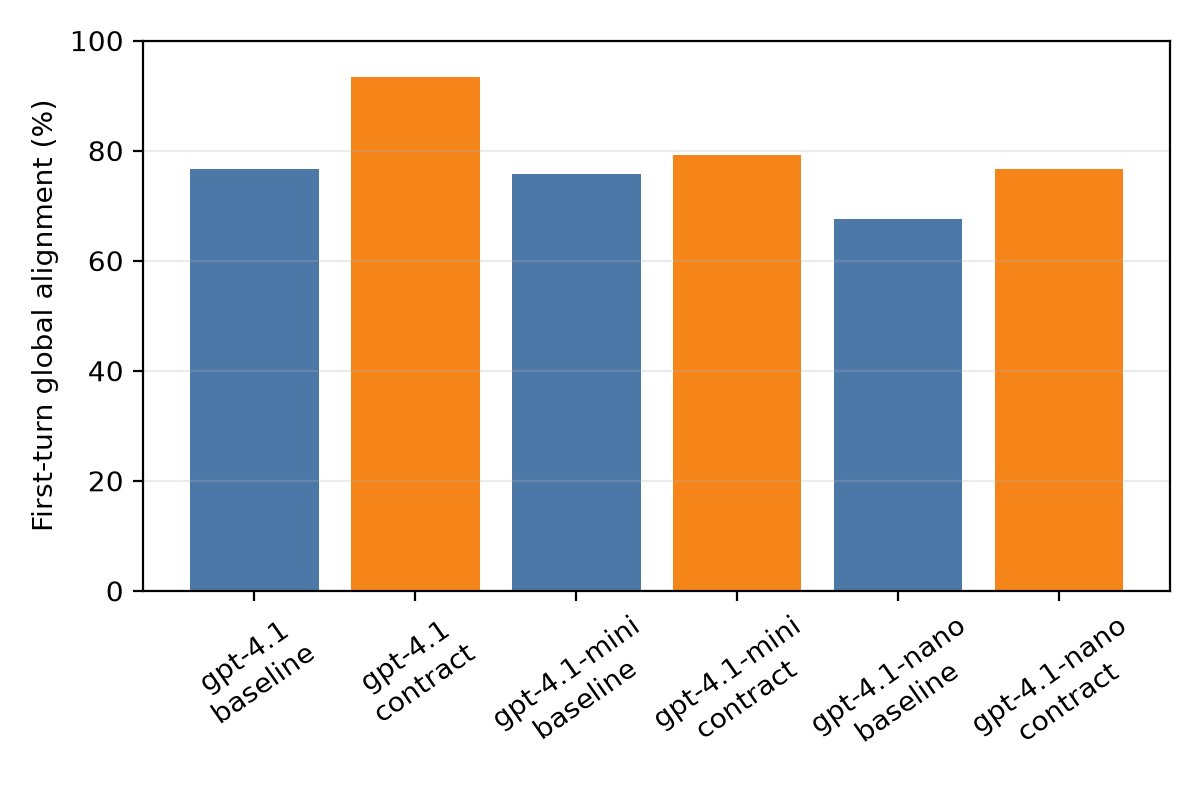
\includegraphics[width=0.98\linewidth]{figures/ftga_by_condition.png}
\caption{First-turn global alignment by model and condition on the 120-item stress pilot.}
\label{fig:ftga}
\end{figure}

Paired sign-test sensitivity supports the strongest mitigation effects while
clarifying the weaker mini result. For GPT-4.1, the contract improves FTGA on
20 paired items, worsens none, and ties on 100 items ($p<0.0001$); mean RTT
falls by 0.133 and mean token tax by 0.300. For nano, FTGA improves on 12 items,
worsens on 1, and ties on 107 ($p=0.0034$); mean RTT falls by 0.142 and token
tax by 0.351. Mini's FTGA movement is smaller: 4 improved, 0 worsened, and 116
tied ($p=0.125$), although token-tax reduction is consistent.

\subsection{Failure families}

\begin{table}[t]
\centering
\small
\begin{tabular}{lrrrr}
\toprule
Task family & Baseline FTGA & Contract FTGA & Baseline fail. & Contract fail. \\
\midrule
Editing preservation & 33.3 & 70.0 & 60/90 & 27/90 \\
Output-language inference & 100.0 & 100.0 & 0/90 & 0/90 \\
Quote preservation & 90.0 & 91.1 & 9/90 & 8/90 \\
Script/register/locale & 70.0 & 71.1 & 27/90 & 26/90 \\
\bottomrule
\end{tabular}
\caption{Family-level first-turn alignment aggregated across the three models. Editing preservation is the dominant source of baseline burden; output-language inference is saturated in this pilot.}
\label{tab:families-results}
\end{table}

The main burden comes from implicit editing preservation, not from generic
multilingual output-language inference. Table~\ref{tab:families-results} shows
that aggregate baseline FTGA is only 33.3\% for editing preservation, with
60/90 first-turn failures across models. In contrast, output-language inference
is saturated at 100.0\% FTGA in this particular pilot. The contract improves
editing-preservation FTGA to 70.0\%, reducing mean RTT for that family from
0.667 to 0.300. The family-level effect is largest for \texttt{gpt-4.1}
(+63.3 points on editing preservation), followed by nano (+33.3) and mini
(+13.3).

The component breakdown explains why editing preservation is difficult. In
baseline editing-preservation rows, the first-turn language check passes only
33.3\% of the time and the script check passes 66.7\%. Under the contract, those
rates rise to 70.0\% and 92.2\%, respectively. However, preservation pass rates
barely move in some other families, and script/register/locale preservation
remains below saturation. This suggests that the contract helps models separate
instruction language from content language, but it does not fully solve literal
span preservation.

\subsection{Language slices and item consistency}

The aggregate gain is not evenly distributed across language pairs. Averaged
across models, FTGA increases by +20.0 points on Arabic-English, +9.2 points on
Spanish-English, and +0.0 points on Hindi-English. This does not mean that
Hindi-English is easier in general; in this stress pilot, the Hindi-English
slice has little room to improve because baseline FTGA is already high for all
three models. The strongest language-slice improvements are GPT-4.1 on
Arabic-English and Spanish-English (+25.0 points each) and nano on
Arabic-English (+25.0 points). The weakest slice is Spanish-English on
\texttt{gpt-4.1-mini}, where FTGA delta is +0.0 points despite lower token tax.

Item-consistency analysis separates systematic hard items from scattered
one-model failures. Under baseline prompting, 40/120 items fail for at least one
model and 27/120 fail for all three. Under the contract, 35/120 items still fail
for at least one model, but only 8/120 fail for all three. The contract reduces
the number of failing models on 22/120 items and increases it on only 1/120
item. The hardest residual items are concentrated in script/register/locale
rows requiring exact preservation of local literal spans.

\subsection{Repair dynamics and token burden}

Repair trajectories reveal a distinction between first-turn usability and
recoverability. For GPT-4.1, the contract changes the distribution from 92
first-turn successes and 28 initial failures to 112 first-turn successes and 8
initial failures. For nano, first-turn successes rise from 81 to 92 and
unresolved trajectories fall from 7 to 5. Mini has a deliberately modest
trajectory shift: 91 to 95 first-turn successes, with 5 paired RTT improvements,
1 worsening, and 114 ties.

Token tax decreases for all three models, but absolute token burden increases
because the contract prompt is longer. For GPT-4.1, mean total tokens rise from
132.7 under baseline to 256.3 under the contract, even though mean extra tokens
after the first turn decrease from 51.2 to 32.9 and token tax falls from
1.43$\times$ to 1.13$\times$. This is why we interpret token tax as a normalized
repair-burden metric rather than as a cost-saving claim. Future evaluations
should report both normalized repair cost and absolute cost.

\subsection{Prompt controls and mechanism evidence}

We also run single-model prompt diagnostics on \texttt{gpt-4.1-nano}. A longer
generic-helpfulness prompt improves FTGA from 67.5\% to 75.0\%, suggesting that
some mitigation benefit comes from generic instruction-following scaffolding.
The Global Interaction Contract reaches 76.7\% FTGA and the lowest token tax in
that three-condition control. A narrower content-preservation prompt performs
best in a later ablation: 80.0\% FTGA, 0.27 mean RTT, and 1.28$\times$ token tax.
This is an important claim boundary. The three-model paper-facing intervention
is the full Global Interaction Contract, but the best nano prompt tested is the
narrower content-preservation scaffold. The result suggests that content
language and literal-preservation rules drive much of the mitigation.

\subsection{Scorer sensitivity and audit}

Scorer-ablation diagnostics show that the headline trend is not caused by one
fragile automatic rule. Relaxing language alone would move aggregate baseline
FTGA from 73.3\% to 76.4\%; relaxing preservation alone would move it to 78.9\%;
relaxing task alone would not change it. Under the contract, relaxing language
would move FTGA from 83.1\% to 83.3\%, and relaxing preservation would move it
to 88.3\%. Many failures violate multiple checks at once, especially editing
failures that combine language, script, and task violations.

The blinded judge audit agrees with the corrected automatic scorer on 71/72
sampled pass/fail labels (98.6\%; Wilson 95\% CI 92.5--99.8). The single
pass/fail disagreement is an editing-preservation response where the automatic
scorer rejects Spanish framing around English rewrites while the judge accepts
the answer. Component agreement is lower for preservation and register/locale,
which reinforces our conservative claim: the LLM judge is useful as a scorer
sanity check, but native/near-native validation remains necessary before making
stronger cultural or register claims.
